\documentclass{../../../oss-apphys-exam}
\newcounter{last}

\begin{document}

\gentitle{3}{GAUSS'S LAW, PART 1}

\raggedcolumns

\runningheader{
  \fontfamily{phv}\small
  \textcolor{gray}{AP PHYSICS C: ELECTRICITY AND MAGNETISM $\blacksquare$}
  \textbf{MULTIPLE-CHOICE QUESTIONS}}{}{}


\begin{multicols*}{2}
  \begin{questions}

    \question A non-conducting sphere does not have a uniform charge density,
    but the density $\rho$ varies with the distance $r$ from the center of the
    sphere according to the equation $\rho=\beta r$ where $\beta$ is a positive
    constant. The electric field inside the sphere ($r<R$) at a distance $r$
    from the center of the sphere is
    \begin{choices}
      \choice $\dfrac{\beta r^2}{12\epsilon_0}$
      \choice $\dfrac{\beta r^2}{3\epsilon_0}$
      \choice $\dfrac{\beta r}{2\epsilon_0}$
      \choice $\dfrac{\beta r^2}{2\epsilon_0}$
      \choice $\dfrac{\beta r^2}{4\epsilon_0}$
    \end{choices}
 
    \question What is the electric potential difference between center and the
    outside surface of the sphere?
    \begin{choices}
      \choice $\dfrac{\beta R^3}{12\epsilon_0}$
      \choice $\dfrac{\beta R}{2\epsilon_0}$
      \choice $\dfrac{\beta R^3}{3\epsilon_0}$
      \choice $\dfrac{\beta R^2}{2\epsilon_0}$
      \choice $\dfrac{\beta R^2}{4\epsilon_0}$
    \end{choices}
    
    \question According to Gauss's law, which of the following statements is
    true?
    \begin{choices}
      \choice It is possible to have a nonzero electric field, but zero electric
      flux.
      \choice It is possible to have a nonzero electric flux, but zero electric
      field.
      \choice It is possible to have a nonzero electric flux through a closed
      surface even if the enclosed charge in a surface is zero.
      \choice If a surface is not closed (such as a sheet of paper), the flux
      through it must be zero.
      \choice It is possible for charges located outside a closed surface to
      produce a net positive flux through the surface.
    \end{choices}
    \columnbreak
    
    \question According to Gauss's law, the net electric flux passing through a
    closed surface is
    \begin{choices}
      \choice positive if the flux is entering the surface
      \choice negative if the flux is exiting the surface
      \choice positive if the net charge inside the surface is zero
      \choice negative if the net charge inside the surface is zero
      \choice zero if the net charge inside the surface is zero
    \end{choices}
    
%    \question Gauss's law is most convenient to use when calculating an electric
%    field due to
%    \begin{choices}
%      \choice charges outside a closed surface
%      \choice charges inside a closed surface that has high symmetry
%      \choice charges inside a closed surface that has low symmetry
%      \choice a potential difference that is negative
%      \choice a potential difference that is positive
%    \end{choices}
%    \columnbreak
    
    \uplevel{
      \textbf{Question \ref{cube1}-\ref{cube2}}
      \cpic{.3}{cube}
    }
    \question A cube has sides of length $a$. The cube rests so that one side
    rests on the $x$-axis as shown. An electric field is established in the
    $x$-direction according to the function $E_x=bx^2$ , where $b$ is a positive
    constant. Which of the following statements is true?
    \label{cube1}
    \begin{choices}
      \choice There is a net charge inside the cube.
      \choice There is no net charge inside the cube.
      \choice The flux passing through the cube is negative.
      \choice The flux passing through the cube is zero.
      \choice The flux diminishes while passing through the cube.
    \end{choices}
    
    \question The charge inside the cube can be expressed by the equation
    \label{cube2}
    \begin{choices}
      \choice $\epsilon_0ba$
      \choice $\epsilon_0ba^2$
      \choice $\epsilon_0ba^3$
      \choice $\epsilon_0ba^4$
      \choice $\epsilon_0b^22a^2$
    \end{choices}
   
%    \uplevel{
%      \textbf{Questions \ref{sphere1}--\ref{sphere2}}: A nonconducting spherical
%      charge distribution has a nonuniform positive charge density $\rho$. The
%      center of the sphere is point $O$, the radius of the sphere is $a$. The
%      sphere is centered on the $x$-axis. A point inside the sphere lies on
%      the $x$-axis at a distance $x_1$ from the center of the sphere. Another
%      point, $x_2$, is outside the sphere on the $x$-axis.
%      \begin{center}
%        \begin{tikzpicture}
%          \draw[thick] circle(1);
%          \fill circle(.08);
%          \draw[very thick,->](0,0)--(0,1) node[midway,left]{$a$};
%          \draw[dashed,thick] (0,0)--(6,0) node[right]{\small$\infty$};
%          \fill(.5,0) circle(.05) node[below]{\footnotesize$x_1$};
%          \fill(4,0)  circle(.05) node[below]{\footnotesize$x_2$};
%        \end{tikzpicture}
%      \end{center}
%    }
%
%    \question The electric field at point $x_2$ can be determined by
%    \begin{choices}
%      \choice using Gauss's law to determine the electric field from $O$ to $a$,
%      then using Gauss's law to determine the electric field from $a$ to $x_2$,
%      then finding the difference between the two electric fields.
%      \choice using Gauss's law to determine the electric field from $O$ to $a$,
%      then using Gauss's law to determine the electric field from $a$ to $x_2$,
%      then finding the sum of the two electric fields.
%      \choice integrating the electric potential outside the sphere from
%      infinity to $a$, then integrating the electric potential inside the
%      sphere from $a$ to $x_1$, then finding the difference between the two
%      potential integrals.
%      \choice integrating the electric potential outside the sphere from
%      infinity to $a$, then integrating the electric potential inside the
%      sphere from $a$ to $x_1$, then finding the sum of the two potential
%      integrals.
%      \choice determining the derivative of the potential function inside and
%      outside the sphere, then finding the difference between the two
%      derivatives.
%    \end{choices}
%    \label{sphere1}
%    \vspace{.7in}
%    
%    \question The electric potential at point $x_1$ can be determined by
%    \begin{choices}
%      \choice determining the derivative of the electric field function inside
%      and outside the sphere, then finding the difference between the two
%      derivatives.
%      \choice determining the derivative of the electric field function inside
%      and outside the sphere, then finding the sum of the two derivatives.
%      \choice integrating the derivative of the product of the electric field
%      and potential functions, then finding their sum.
%      \choice integrating the electric field outside the sphere from infinity
%      to $a$, then integrating the electric field inside the sphere from $a$ to
%      $x_1$, then finding the sum of the two potentials.
%      \choice integrating the electric field outside the sphere from infinity
%      to $a$, then integrating the electric field inside the sphere from $a$ to
%      $x_1$, then finding the difference between the two potentials.
%    \end{choices}
%    \label{sphere2}
%    \vspace{.7in}
    \columnbreak
    
    \uplevel{
      \textbf{Questions \ref{solid1}--\ref{solid2}}: A solid conducting sphere
      of radius $a$ is placed inside a conducting spherical shell of radius
      $3a$, as shown. A charge $+2Q$ is placed on the inner sphere, and a
      charge $-Q$ is placed on the outer sphere.
      \begin{center}
        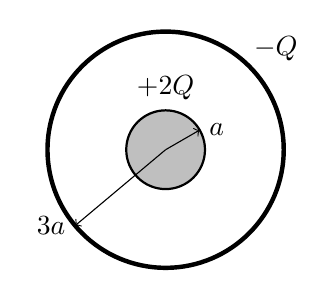
\begin{tikzpicture}[scale=.5]
          \fill circle(.07);
          \draw[thick,fill=lightgray] circle(1);
          \node[thick,above] at (0,1) {$+2Q$};
          \draw[ultra thick] circle(3);
          \node[above right] at (2,2) {$-Q$};
          \draw[rotate=30,->](0,0)--(1,0)node[right]{$a$};
          \draw[rotate=220,->](0,0)--(3,0)node[left]{$3a$};
        \end{tikzpicture}
      \end{center}
    }
    
    \question Which of the following graphs best represents the electric field
    $\vec E$ as a function of the distance $r$ from the center of the spheres?

    \begin{oneparchoices}
      \choice
      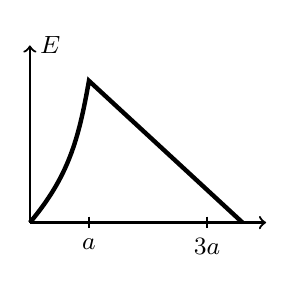
\begin{tikzpicture}[scale=1.5]
        \begin{scope}[thick]
          \draw[->](0,0)--(2,0);
          \draw[->](0,0)--(0,1.5) node[right]{\small$E$};
          \draw(.5,.05)--(.5,-.05) node[below]{\small$a$};
          \draw(1.5,.05)--(1.5,-.05) node[below]{\small$3a$};
        \end{scope}
        \draw[ultra thick](0,0) to[out=50,in=260](.5,1.2)--(1.8,0);
      \end{tikzpicture}
      \choice
      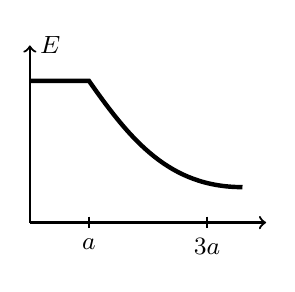
\begin{tikzpicture}[scale=1.5]
        \begin{scope}[thick]
          \draw[->](0,0)--(2,0);
          \draw[->](0,0)--(0,1.5) node[right]{\small$E$};
          \draw(.5,.05)--(.5,-.05) node[below]{\small$a$};
          \draw(1.5,.05)--(1.5,-.05) node[below]{\small$3a$};
        \end{scope}
        \draw[ultra thick](0,1.2)--(.5,1.2) to[out=-55,in=180](1.8,.3);
      \end{tikzpicture}
      \choice
      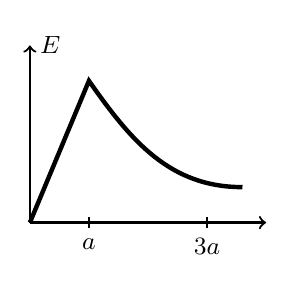
\begin{tikzpicture}[scale=1.5]
        \begin{scope}[thick]
          \draw[->](0,0)--(2,0);
          \draw[->](0,0)--(0,1.5) node[right]{\small$E$};
          \draw(.5,.05)--(.5,-.05) node[below]{\small$a$};
          \draw(1.5,.05)--(1.5,-.05) node[below]{\small$3a$};
        \end{scope}
        \draw[ultra thick](0,0)--(.5,1.2) to[out=-55,in=180](1.8,.3);
      \end{tikzpicture}
      \choice
      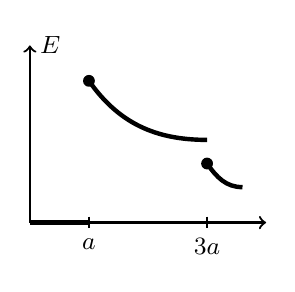
\begin{tikzpicture}[scale=1.5]
        \draw[thick,->](0,0)--(2,0);
        \draw[thick,->](0,0)--(0,1.5) node[right]{\small$E$};
        \draw[thick](.5,.05)--(.5,-.05) node[below]{\small$a$};
        \draw[thick](1.5,.05)--(1.5,-.05) node[below]{\small$3a$};
        \draw[ultra thick](0,0)--(.5,0);
        \draw[ultra thick](0.5,1.2) to[out=-55,in=180](1.5,.7);
        \draw[ultra thick](1.5,.5) to[out=-55,in=180](1.8,.3);
        \fill(.5,1.2) circle(.05);
        \fill(1.5,.5) circle(.05);
      \end{tikzpicture}
      \choice
      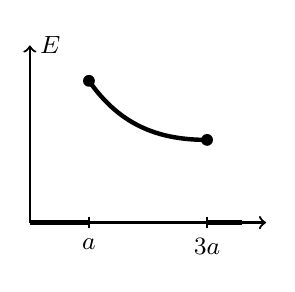
\begin{tikzpicture}[scale=1.5]
        \draw[thick,->](0,0)--(2,0);
        \draw[thick,->](0,0)--(0,1.5) node[right]{\small$E$};
        \draw[thick](.5,.05)--(.5,-.05) node[below]{\small$a$};
        \draw[thick](1.5,.05)--(1.5,-.05) node[below]{\small$3a$};
        \draw[ultra thick](0,0)--(.5,0);
        \draw[ultra thick](0.5,1.2) to[out=-55,in=180](1.5,.7);
        \draw[ultra thick](1.5,0)--(1.8,0);
        \fill(.5,1.2) circle(.05);
        \fill(1.5,.7) circle(.05);
      \end{tikzpicture}
    \end{oneparchoices}
    \label{solid1}
    \columnbreak
    
    \question Which of the following graphs best represents the electric
    potential $V$ as a function of the distance $r$ from the center of the
    spheres?

    \begin{oneparchoices}
      \choice
      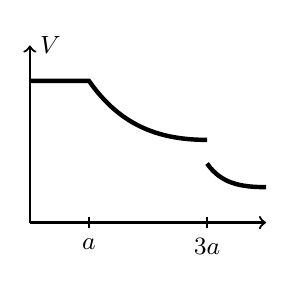
\begin{tikzpicture}[scale=1.5,thick]
        \draw[->](0,0)--(2,0);
        \draw[->](0,0)--(0,1.5) node[right]{\small$V$};
        \draw(.5,.05)--(.5,-.05) node[below]{\small$a$};
        \draw(1.5,.05)--(1.5,-.05) node[below]{\small$3a$};
        \draw[ultra thick](0,1.2)--(.5,1.2) to[out=-55,in=180](1.5,.7);
        \draw[ultra thick](1.5,.5) to[out=-55,in=180](2,.3);
      \end{tikzpicture}
      \choice
      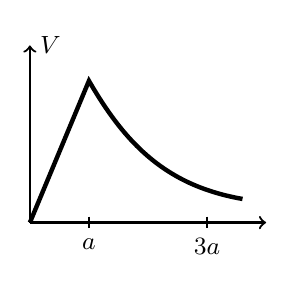
\begin{tikzpicture}[scale=1.5,thick]
        \draw[->](0,0)--(2,0);
        \draw[->](0,0)--(0,1.5) node[right]{\small$V$};
        \draw(.5,.05)--(.5,-.05) node[below]{\small$a$};
        \draw(1.5,.05)--(1.5,-.05) node[below]{\small$3a$};
        \draw[ultra thick](0,0)--(.5,1.2)to[out=-60,in=170](1.8,.2);
      \end{tikzpicture}
      \choice
      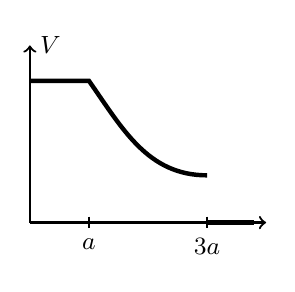
\begin{tikzpicture}[scale=1.5,thick]
        \draw[->](0,0)--(2,0);
        \draw[->](0,0)--(0,1.5) node[right]{\small$V$};
        \draw(.5,.05)--(.5,-.05) node[below]{\small$a$};
        \draw(1.5,.05)--(1.5,-.05) node[below]{\small$3a$};
        \draw[ultra thick](0,1.2)--(.5,1.2) to[out=-55,in=180](1.5,.4);
        \draw[ultra thick](1.5,0)--(1.9,0);
      \end{tikzpicture}
      \choice
      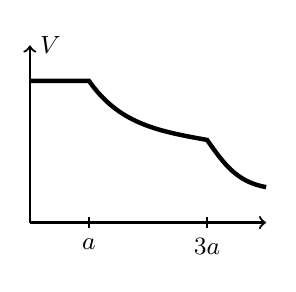
\begin{tikzpicture}[scale=1.5,thick]
        \draw[->](0,0)--(2,0);
        \draw[->](0,0)--(0,1.5) node[right]{\small$V$};
        \draw(.5,.05)--(.5,-.05) node[below]{\small$a$};
        \draw(1.5,.05)--(1.5,-.05) node[below]{\small$3a$};
        \draw[ultra thick](0,1.2)--(.5,1.2)
        to[out=-55,in=170](1.5,.7) to[out=-55,in=170](2,.3);
      \end{tikzpicture}
      \choice
      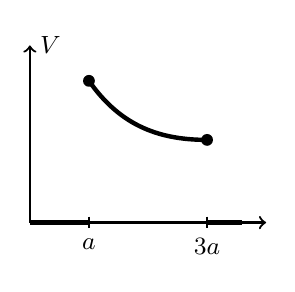
\begin{tikzpicture}[scale=1.5,thick]
        \draw[->](0,0)--(2,0);
        \draw[->](0,0)--(0,1.5) node[right]{\small$V$};
        \draw(.5,.05)--(.5,-.05) node[below]{\small$a$};
        \draw(1.5,.05)--(1.5,-.05) node[below]{\small$3a$};
        \draw[ultra thick](0,0)--(.5,0);
        \draw[ultra thick](0.5,1.2) to[out=-55,in=180](1.5,.7);
        \draw[ultra thick](1.5,0)--(1.8,0);
        \fill(.5,1.2) circle(.05);
        \fill(1.5,.7) circle(.05);
      \end{tikzpicture}   
    \end{oneparchoices}
    \label{solid2}
  \end{questions}
  \setcounter{last}{\value{question}}
\end{multicols*}
\newpage


\runningheader{
  \fontfamily{phv}\small
  \textcolor{gray}{AP PHYSICS C: ELECTRICITY AND MAGNETISM $\blacksquare$}
  \textbf{FREE-RESPONSE QUESTIONS}}{}{}

% TAKEN FROM 2007 AP PHYSICS C EXAM FREE-RESPONSE QUESTION E&M 2
\begin{center}
  \begin{tikzpicture}[thick,scale=.7]
    \draw[fill=gray!50] circle (3) node[below=45]{\small$-Q$};
    \draw[fill=white] circle (2);
    \draw[fill=gray!50] circle (1) node[below=5]{\small$+Q$};
    
    \fill[rotate=125] (1,0) circle (.075) node[above left=-3]{\small$X$};
    \fill[rotate=120] (2,0) circle (.075) node[below right=-2.5]{\small$Y$};

    \draw[axes,rotate=70] (0,0)--(1,0) node[pos=.7,left=-2]{\small$a$};
    \draw[axes,rotate=25] (0,0)--(2,0) node[pos=.7,above=-1]{\small$2a$};
    \draw[axes,rotate=-25] (0,0)--(3,0) node[pos=.9,above=-1]{\small$3a$};
  \end{tikzpicture}
\end{center}
\begin{questions}
  \setcounter{question}{\value{last}}
  
  \question In the figure above, a nonconducting solid sphere of radius a with
  charge $+Q$ uniformly distributed throughout its volume is concentric with a
  nonconducting spherical shell of inner radius $2a$ and outer radius $3a$ that
  has a charge $-Q$ uniformly distributed throughout its volume. Express all
  answers in terms of the given quantities and fundamental constants.

  \begin{parts}
    \part Using Gauss's law, \textbf{derive} expressions for the magnitude of
    the electric field as a function of radius $r$ in the following regions.
    \begin{subparts}
      \subpart Within the solid sphere ($r<a$)
      \vspace{\stretch1}
      
      \subpart Between the solid sphere and the spherical shell ($a<r<2a$)
      \vspace{\stretch1}
      
      \subpart Within the spherical shell ($2a<r<3a$)
      \vspace{\stretch3}
      \newpage
      
      \subpart Outside the spherical shell ($r>3a$)
      \vspace{\stretch1}
    \end{subparts}
    
    \part What is the electric potential at the outer surface of the spherical
    shell ($r=3a$)? \textbf{Explain} your reasoning.
    \vspace{\stretch2}
    
    \part\textbf{Derive} an expression for the electric potential difference
    $V_X-V_Y$ between points $X$ and $Y$ shown in the figure.
    \vspace{\stretch3}
  \end{parts}
  \newpage

  % TAKEN FROM 2019 AP PHYSICS C E&M EXAM FREE-RESPONSE QUESTION 2. THE QUESTION
  % HAS BEEN SLIGHTLY MODIFIED TO FIT THE FORMATTING STANDARD SINCE 2024
  \uplevel{
    \centering
    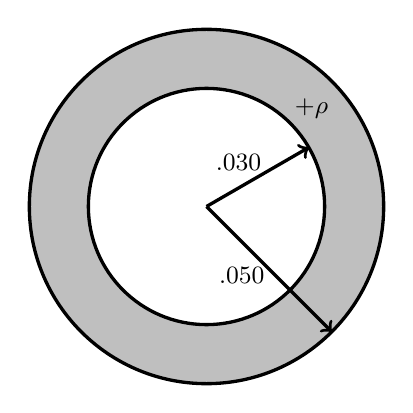
\begin{tikzpicture}[very thick,scale=.75]
      \draw[fill=gray!50] circle (3) node[above right=28]{\small$+\rho$};
      \draw[fill=white] circle (2);
      
      \draw[->,rotate=-45](0,0)--(3,0)
      node[pos=.55,left]{\small\SI{.050}\metre};

      \draw[->,rotate=30](0,0)--(2,0)
      node[pos=.75,left=4]{\small\SI{.030}\metre};
    \end{tikzpicture}
  }

  \question A nonconducting hollow sphere of inner radius \SI{.030}{\metre} and
  outer radius \SI{.050}{\metre} carries a positive volume charge density
  $\rho$, as shown in the figure above. The charge density $\rho$ of the sphere
  is given as a function of the distance $r$ from the center of the sphere, in
  meters, by the following.
  \begin{align*}
    r<\SI{.030}\metre:\quad\quad & \rho = 0\\
    \SI{.030}\metre<r<\SI{.050}\metre:\quad\quad & \rho = \frac br\quad\quad
    \text{where}\quad\quad b = \SI{1.6e-6}{\coulomb\per\metre\squared}\\
    r > \SI{.050}\metre:\quad\quad & \rho = 0
  \end{align*}
  \begin{parts}
    \part\textbf{Calculate} the total charge of the sphere.
    \vspace{\stretch1}
    
    \part Using Gauss's law, \textbf{calculate} the magnitude of the electric
    field $E$ at the outer surface of the sphere.
    \vspace{\stretch1}
    \newpage
    
    \part On the axes below, \textbf{sketch} the magnitude of the electric
    field $E$ as a function of distance $r$ from the center of the sphere.
    \uplevel{
      \centering
      \begin{tikzpicture}[scale=.9]
        \draw[axes] (0,0)--(10,0) node[right]{$r$ [m]};
        \draw[axes] (0,0)--(0,6) node[above]{$E$};

        \draw[dashed] (4,-.2)--(4,5) node[pos=0,below]{\SI{.030}\metre};
        \draw[dashed] (7,-.2)--(7,5) node[pos=0,below]{\SI{.050}\metre};
      \end{tikzpicture}
    }

    \part\textbf{Calculate} the electric potential $V$ at the outer surface of
    the sphere. Assume the electric potential to be zero at infinity.
    \vspace{\stretch1}
    
    \uplevel{
      A proton is released from rest at the outer surface of the sphere at
      time $t=0$.
    }
    \part\textbf{Calculate} the magnitude of the initial acceleration of the
    proton.
    \vspace{\stretch1}
    
    \part\textbf{Calculate} the speed of the proton after a long time.
    \vspace{\stretch1}
  \end{parts}
  \newpage

  % TAKEN FROM 2012 AP PHYSICS C E&M EXAM FREE-RESPONSE QUESTION 1. THE
  % TIKZ FIGURE BELOW IS A FAIRLY GOOD REPRODUCTION OF THE ORIGINAL AP EXAM
  % DIAGRAM. ALSO, THE FORMATTING OF THE QUESTIONS HAS BEEN MODIFIED TO CONFORM
  % TO THE NEWER STANDARD SINCE 2025
  \uplevel{
    \centering
    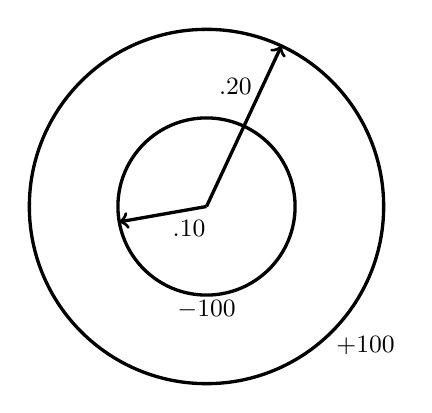
\begin{tikzpicture}[very thick,scale=.75]
      \draw circle (3) node[below right=43]{\small$+\SI{100}\volt$};
      \draw[fill=white] circle (1.5) node[below=30]{\small$\SI{-100}\volt$};

      \draw[->,rotate=190] (0,0)--(1.5,0)
      node[pos=.2,below]{\small\SI{.10}\metre};

      \draw[->,rotate=65] (0,0)--(3,0) node[pos=.75,left]{\small\SI{.20}\metre};
    \end{tikzpicture}
  }
  
  \question Two thin, concentric, conducting spherical shells, insulated from
  each other, have radii of \SI{.10}{\metre} and \SI{.20}{\metre}, as shown
  above. The inner shell is set at an electric potential of \SI{-100}\volt, and
  the outer shell is set at an electric potential of $+\SI{100}\volt$, with each
  potential defined relative to the conventional reference point. Let $Q_i$ and
  $Q_o$ represent the net charge on the inner and outer shells, respectively,
  and let $r$ be the radial distance from the center of the shells. Express all
  algebraic answers in terms of $Q_i$, $Q_o$, $r$, and fundamental constants,
  as appropriate.
  \begin{parts}
    \part Using Gauss's Law, \textbf{derive} an algebraic expression for the
    electric field $E(r)$ for $\SI{.10}\metre<r<\SI{.20}\metre$.
    \vspace{\stretch1}
    
    \part\textbf{Determine} an algebraic expression for the electric field
    $E(r)$ for   $r>\SI{.20}\metre$.
    \vspace{\stretch1}
    
    \part\textbf{Determine} an algebraic expression for the electric potential
    $V(r)$ for $r>\SI{.20}\metre$.
    \vspace{\stretch1}
    
    \part Using the numerical information given, \textbf{calculate} the value
    of the total charge $Q_T$ on the two spherical shells ($Q_T = Q_i + Q_o$).
    \vspace{\stretch1}
    \newpage
    
    \part On the axes below, \textbf{sketch} the electric field $E$ as a
    function of $r$. Let the positive direction be radially outward.
    \uplevel{
      \centering
      \begin{tikzpicture}
        \draw[axes] (0,0)--(8,0) node[right]{$r$ [m]};
        \draw[axes] (0,-2.5)--(0,2.5) node[above]{$E$};
        \foreach \x in {0.10,0.20,0.30} \draw (\x*20,.1)--+(0,-.2)
        node[below]{$\x$};
      \end{tikzpicture}
    }

    \part On the axes below, \textbf{sketch} the electric potential $V$ as a
    function of $r$.
    \uplevel{
      \centering
      \begin{tikzpicture}
        \draw[axes] (0,0)--(8,0) node[right]{$r$ [m]};
        \draw[axes] (0,-2.5)--(0,2.5) node[above]{$V$};
        \foreach \x in {0.10,0.20,0.30} \draw (\x*20,.1)--+(0,-.2)
        node[below]{$\x$};
      \end{tikzpicture}
  }
   \end{parts}
  \newpage

  
  % TAKEN FROM 2003 AP PHYSICS C EXAM FREE-RESPONSE QUESTION E&M 1. THE
  % TIKZ FIGURE BELOW IS A FAIRLY GOOD REPRODUCTION OF THE ORIGINAL AP EXAM
  % DIAGRAM.
  \uplevel{
    \centering
    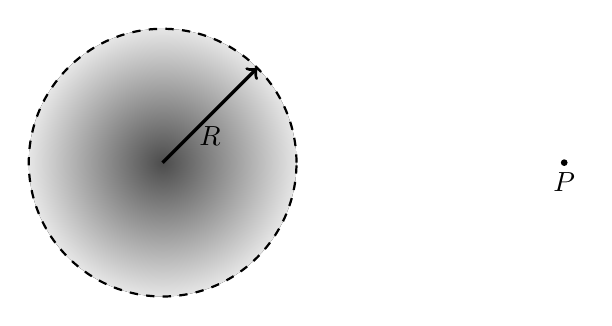
\begin{tikzpicture}[scale=.85]
      \filldraw[dashed,thick,
        even odd rule,
        inner color=black!70,
        outer color=gray!20] circle (2);
      \draw[very thick,->,rotate=45](0,0)--(2,0) node[midway,below]{$R$};
      \fill(6,0) circle(.05) node[below]{$P$};
    \end{tikzpicture}
  }
  \question A spherical cloud of charge of radius $R$ contains a total charge
  $+Q$ with a nonuniform volume charge density that varies according to the
  equation
  \begin{align*}
    \rho(r)&= \rho_0\left( 1 -\dfrac rR \right)\text{ for }r\leq R\text{ and}\\
    \rho(r)&= 0\text{ for }r>R
  \end{align*}
  where $r$ is the distance from the center of the cloud. Express all algebraic
  answers in terms of $Q$, $R$, and fundamental constants.
  \begin{parts}
    \part\textbf{Determine} the following as a function of $r$ for $r>R$.
    \begin{subparts}
      \subpart The magnitude $E$ of the electric field
      \vspace{\stretch1}
      
      \subpart The electric potential $V$ (You may assume that $V(\infty)=0$)
      \vspace{\stretch1}
    \end{subparts}
    \part A proton is placed at point $P$ shown above and released.
    \textbf{Describe} its motion for a long time after its release.
    \vspace{\stretch1}
    \newpage
    
    \part An electron of charge magnitude $e$ is now placed at point $P$, which
    is a distance $r$ from the center of the sphere, and released.
    \textbf{Determine} the kinetic energy of the electron as a function of $r$
    as it strikes the cloud.
    \vspace{\stretch1}
    
    \part\textbf{Derive} an expression for $\rho_0$.
    \vspace{\stretch1}
    
    \part\textbf{Determine} the magnitude $E$ of the electric field as a
    function of $r$ for $r\leq R$.
    \vspace{\stretch3}
  \end{parts}
  \newpage

  % TAKEN FROM 2014 AP PHYSICS C E&M EXAM FREE-RESPONSE QUESTION 1. THE
  % FORMATTING OF THE QUESTIONS HAS BEEN MODIFIED TO CONFORM TO THE NEWER
  % STANDARD SINCE 2025
  
  \question A scientist describes an electrically neutral atom with a model
  that consists of a nucleus that is a point particle with positive charge $+Q$
  at the center of the atom and an electron volume charge density of the form
  \begin{displaymath}
    \rho(r)=
    \begin{cases}
      -\dfrac\beta{r^2}e^{-\frac{-r}\alpha} & r<\alpha\\
      0          & r>\alpha
      \end{cases}
  \end{displaymath}
  where $\alpha$ and $\beta$ are positive constants and $r$ is the distance
  from the center of the atom.
  
  \begin{parts}
    \part On the axes below, let $r$ stand for the radius of a Gaussian
    sphere. \textbf{Sketch} the graph for each of the following charges
    enclosed by the Gaussian sphere as a function of $r$. Explicitly
    \textbf{label} any intercepts, asymptotes, maxima, or minima with numerical
    values or algebraic expressions, as appropriate.
    \begin{subparts}
      \subpart The \underline{nuclear charge} only
      \uplevel{
        \centering
        \begin{tikzpicture}
          \draw[axes] (0,0)--(6,0) node[right]{$r$};
          \draw[axes] (0,-2)--(0,2) node[above]{$q$};
          \draw (.1,1.5)--+(-.2,0) node[left]{$+Q$};
          \draw (.1,-1.5)--+(-.2,0) node[left]{$-Q$};
          \draw (3,.1)--+(0,-.2) node[below]{$\alpha$};
        \end{tikzpicture}
      }
      
      \subpart The \underline{electron charge} only
      \uplevel{
        \centering
        \begin{tikzpicture}
          \draw[axes] (0,0)--(6,0) node[right]{$r$};
          \draw[axes] (0,-2)--(0,2) node[above]{$q$};
          \draw (.1,1.5)--+(-.2,0) node[left]{$+Q$};
          \draw (.1,-1.5)--+(-.2,0) node[left]{$-Q$};
          \draw (3,.1)--+(0,-.2) node[below]{$\alpha$};
        \end{tikzpicture}
      }
    \end{subparts}

    \part The dashed curve on the graph below represents the electric field as
    a function of distance $r$ due to the positive nucleus of the atom without
    any electrons. The nucleus is modeled as a point particle of charge $+Q$.
    On the same graph, \textbf{sketch} the electric field as a function of
    distance $r$ for the neutral atom as defined by the scientist's model,
    which includes the nucleus and the negative electrons surrounding it.
    \uplevel{
      \centering
      \begin{tikzpicture}
        \draw[axes] (0,0)--(6,0) node[right]{$r$};
        \draw[axes] (0,-2)--(0,2.2) node[above]{$E$};
        \draw[axes,dashed] (.3,1.9) to[out=-80,in=178] (5.5,.07);
        \draw (3,.1)--+(0,-.2) node[below]{$\alpha$};
      \end{tikzpicture}
    }
    \newpage
    
    \part Use Gauss's law to \textbf{derive} an expression for the electric
    field strength due to the neutral atom for the following positions in terms
    of $Q$, $\alpha$, $\beta$, $r$, and fundamental constants, as appropriate.
    \begin{subparts}
      \subpart $r > \alpha$
      \subpart $r < \alpha$
    \end{subparts}
    \vspace{\stretch3}
    
    \part Based on the model proposed by the scientist, \textbf{explain} the
    physical meaning of the constant $\alpha$.
    \vspace{\stretch1}
  \end{parts}
  \newpage

  % TAKEN FROM 2022 AP PHYSICS C E&M EXAM FREE-RESPONSE QUESTION 1. WE ARE STILL
  % USING THE ORIGINAL DIAGRAM FROM THE TEST ITSELF, BUT THE FORMATTING OF THE
  % QUESTIONS HAS BEEN MODIFIED TO CONFORM TO THE NEWER STANDARD SINCE 2025
  \uplevel{
    \centering
    \pic{.65}{concentric-spheres}

    \underline{Note:} Figures not drawn to scale.
  }
  \question A nonconducting sphere of uniform volume charge density is
  surrounded by a thin concentric conducting spherical shell, as shown in the
  cutout view. The sphere has a charge of $-Q$ and the shell has a charge of
  $+3Q$. The radii of the inner sphere and spherical shell are $R$ and $4R$,\
  respectively, as shown in the cross-section view.
  \begin{parts}
    \part\textbf{Determine} the charge on the outer surface of the shell.
    \vspace{\stretch1}

    \part Using Gauss's law, \textbf{derive} an expression for the electric
    field a distance $r$ from the center of the sphere for $r<R$. Express your
    answer in terms of $Q$, $R$, $r$, and physical constants, as appropriate.
    \vspace{\stretch1}

    \part The magnitude of the electric field at $r=R$ is
    \SI8{\newton\per\coulomb}. \textbf{Calculate} the value of the electric
    field at $r=2R$.
    \vspace{\stretch1}
    \newpage
    
    \part\textbf{Derive} an expression for the absolute value of the potential
    difference between the outer surface of the sphere and the inner surface of
    the shell. Express your answer in terms of $Q$, $R$, and physical
    constants, as appropriate.
    \vspace{\stretch1}

    \part On the following axes that include regions I, II, and III,
    \textbf{sketch} a graph of the electric field $E$ as a function of the
    distance $r$ from the center of the sphere.
    \uplevel{
      \centering
      \begin{tikzpicture}[scale=.8]
        \draw[axes] (0,0)--(14,0) node[right]{$r$} node[pos=0,left]{$O$};
        \draw[axes] (0,-4)--(0,4) node[above]{$E$};
        \foreach \x in {2.5,10} \draw[dashed] (\x,3.7)--(\x,-4);
        \draw (2.5,.2)--+(0,-.4) node[below,fill=white]{$R$};
        \draw (10,.2)--+(0,-.4) node[below,fill=white]{$4R$};
        \node at (1.25,4) {I};
        \node at (6.25,4) {II};
        \node at (12,4) {III};
      \end{tikzpicture}
    }

    \part On the following axes that include regions I, II, and III,
    \textbf{sketch} a graph of the electric potential $V$ as a function of the
    distance $r$ from the center of the sphere.
    \uplevel{
      \centering
      \begin{tikzpicture}[scale=.8]
        \draw[axes] (0,0)--(14,0) node[right]{$r$} node[pos=0,left]{$O$};
        \draw[axes] (0,-4)--(0,4) node[above]{$V$};
        \foreach \x in {2.5,10} \draw[dashed] (\x,3.7)--(\x,-4);
        \draw (2.5,.2)--+(0,-.4) node[below,fill=white]{$R$};
        \draw (10,.2)--+(0,-.4) node[below,fill=white]{$4R$};
        \node at (1.25,4) {I};
        \node at (6.25,4) {II};
        \node at (12,4) {III};
      \end{tikzpicture}
      
    }
  \end{parts}
  
%  % TAKEN FROM THE 2004 AP PHYSICS C FREE-RESPONSE QUESTION E&M 1. NO CHANGES TO
%  % THE QUESTION HAVE BEEN MADE
%  \uplevel{
%    \cpic{.65}{nonconcentric}
%  }
%  \question The figure above left shows a hollow, infinite, cylindrical,
%  uncharged conducting shell of inner radius $r_1$ and outer radius $r_2$. An
%  infinite line charge of linear charge density $+\lambda$ is parallel to its
%  axis but off center. An enlarged cross section of the cylindrical shell is
%  shown above right.
%  \begin{parts}
%    \part On the cross section above right,
%    \begin{subparts}
%      \subpart sketch the electric field lines, if any, in each of regions I,
%      II, and III and
%      \subpart use $+$ and $-$ signs to indicate any charge induced on the
%      conductor.
%      \end{subparts}
%    \part In the spaces below, rank the electric potentials at points $a$, $b$,
%    $c$, $d$, and $e$ from highest to lowest (1 = highest potential). If two
%    points are at the same potential, give them the same number.
%
%    \vspace{.1in}
%    \underline{\hspace{.2in}} $V_a$\hspace{.3in}
%    \underline{\hspace{.2in}} $V_b$\hspace{.3in}
%    \underline{\hspace{.2in}} $V_c$\hspace{.3in}
%    \underline{\hspace{.2in}} $V_d$\hspace{.3in}
%    \underline{\hspace{.2in}} $V_e$
%    \uplevel{
%      \cpic{.65}{concentric}
%    }
%
%    \part The shell is replaced by another cylindrical shell that has the same
%    dimensions but is nonconducting and carries a uniform volume charge density
%    $+\rho$. The infinite line charge, still of charge density $+\lambda$, is
%    located at the center of the shell as shown above. Using Gauss's law,
%    calculate the magnitude of the electric field as a function of the distance
%    $r$ from the center of the shell for each of the following regions. Express
%    your answers in terms of the given quantities and fundamental constants.
%    \begin{subparts}
%      \subpart $r < r_1$
%      \subpart $r_1\leq r\leq r_2$
%      \subpart $r > r_2$
%    \end{subparts}
%  \end{parts}
  
%\item Two positive charges $+q$ are on the $y$ axis at $y=+a$ and $y=-a$.
%  \begin{enumerate}
%  \item Show that the electric field on the $x$ axis is along the $x$ axis with
%    $E_x=2kqx(x^2+a^2)^{-3/2}$.
%  \item Show that near the origin, when $x\ll a$, $E_x\approx 2kqx/a^3$.
%  \item Show that for $x\gg a$, $E_x\approx 2kq/x^2$.
%  \item Explain why you should expect the result in (c) even before calculating
%    it.
%  \end{enumerate}
%  A bead of mass $m$ with a negative charge $-q$ slides along a thread that
%  runs along the $x$ axis.
%  \begin{enumerate}[resume]
%  \item Show that for small displacements $x\ll a$, the bead experiences a
%    restoring force that is proportional to $x$ and therefore undergoes
%    simple harmonic motion.
%  \item Find the period of the motion.
%  \end{enumerate}
%  %\vspace{\stretch{4}}
%  \newpage
  
%\item Using Gauss's law, find
%  \begin{enumerate}
%  \item the electric field strength inside and outside of a uniformly charged
%    hollow sphere of radius $R$ and surface charge density $\sigma$ (charge
%    per unit area).
%  \item the electric field inside and outside an infinitely long cyclindrical
%    shell of charge of radius $R$ with charge discibution $\sigma$ (charge
%    per unit area).
%  \item the electric field strength inside and outside a infinitely long solid
%    cylinder of radius $R$ carrying a linear uniform charge density $\rho$
%    (charge per unit volume).
%  \end{enumerate}
%  Hint: In all cases, think about where to put the Gaussian surface. Take
%  advantage of symmetry.
%  %\vspace{\stretch{1}}
%  \newpage

%\item For the circuit shown below, find
%  \begin{enumerate}[noitemsep]
%  \item The total equivalent capacitance between the terminals
%  \item The charge stored on each capacitor
%  \item the total stored charge
%  \end{enumerate}
%  \begin{tikzpicture}[scale=1.2,american voltages]
%    \draw[thick] (0,2) to[C=0.30<\micro\farad>,*-] (3,2)
%    to[C=1.0<\micro\farad>] (3,0) to[short,-*](0,0);
%    \draw[thick] (3,2)--(5,2) to[C=0.25<\micro\farad>,] (5,0)--(3,0);
%  \end{tikzpicture}
%  \vspace{\stretch{1}}
  
%\item A parallel-plate capacitor has a capacitance $C_0$ and plate separation
%  of $d$. To dielectric slabs of constants $\kappa_1$ and $\kappa_2$, each of
%  thickness $d/2$ and having the same area as the plates, are inserted between
%  the plates as shown in the figure below. When the free charge on the plates
%  are $Q$,
%  \begin{enumerate}
%  \item find the electric field in each of the dielectric
%  \item find the potential difference between the plates
%  \item show that the new capacitance is given by:
%    $\displaystyle C=\frac{\kappa_1\kappa_2}{\kappa_1+\kappa_2}C_0$
%  \end{enumerate}
%  \pic{.2}{stacked}
%  %\vspace{\stretch{1}}

%\item Several point charges produce the equipotential lines shown.
%  \begin{enumerate}[noitemsep]
%  \item At which point on the diagram is the magnitude of the electric field
%    greatest? Explain.
%  \item Points C and D are approximately \SI{.02}{\metre} apart. Point F is
%    halfway between points C and D. What is the electric field at point F?
%  \item A \SI{5.}{\micro\coulomb} point charge is moved from point C to point
%    E, then to point D by an external force. Determine the work done by the
%    external force.
%  \end{enumerate}
%  \pic{.45}{equipotentials}
%  \vspace{\stretch{1}}

%\item A potential is given by
%  \begin{displaymath}
%    V(x,y,z)=\frac{kQ}{\sqrt{(x-a)^2+y^2+z^2}}
%  \end{displaymath}
%  \begin{enumerate}[noitemsep]
%  \item Find the components $E_x$, $E_y$ and $E_z$ of the electric field by
%    differentiating this potential function.
%  \item What simple charge distribution might be responsible for this potential?
%  \end{enumerate}
%  \vspace{\stretch{1}}
\end{questions}
\end{document}
